% Example taken from:
% C:\Users\anton\Documents\multicomp\examples\1.ursil-build
%
% Multiscale modeling of the morphology and properties of segmented
% silicone-urea copolymers

\documentclass[a4paper]{article}

\usepackage[left=1cm,right=1cm,top=1cm,bottom=1.5cm,bindingoffset=0cm]{geometry}
\usepackage{graphicx}
\usepackage{hyperref}
\usepackage{indentfirst}
\usepackage[utf8]{inputenc}
\usepackage{amsmath}
\usepackage{textcomp}
\usepackage{subcaption}
\usepackage{xcolor}
\usepackage{pgffor}

\usepackage{float}

\usepackage{achemso}


\graphicspath{{./brief_results/}}


\begin{document}


\title{Results of relaxation with different parameters}
\maketitle


\section*{One}

\subsection*{One-one}
pair\_style hybrid/overlay dpd 1 1 34387 \& coul/cut/soft 2 1 5 \& 
lj/cut/soft 2 1 5\newline
pair\_coeff 1 2 coul/cut/soft 0.001\newline
pair\_coeff 3 4 lj/cut/soft 0.05275 10 3 3\newline
pair\_coeff 4 4 lj/cut/soft 0.09150 10 3 3\newline
DPD coefficients: $a_{ij}$ and $r_c$
\begin{figure}[H]\begin{tabular}{llll}
MMT           & Head         & Tail         & Polymer      \\
a=500, r=0.95 & a=500, r=0.8 & a=500, r=0.8 & a=500, r=0.8 \\
              & a=50,  r=0.8 & a=50,  r=0.8 & a=150, r=0.8 \\
              &              & a=50,  r=1   & a=150, r=1   \\
              &              &              & a=150, r=1   \\
\end{tabular}\end{figure}

\begin{figure}[H]
\begin{subfigure}{0.3\textwidth}
  \centering
  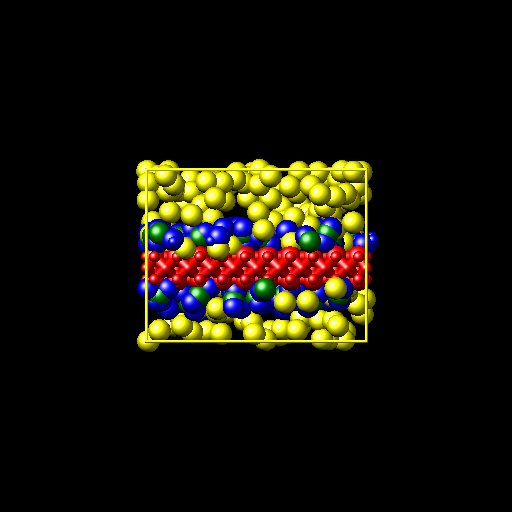
\includegraphics[width=\linewidth,keepaspectratio]{start}
  \caption{}
\end{subfigure}
\begin{subfigure}{0.3\textwidth}
  \centering
  \includegraphics[width=\linewidth,keepaspectratio]{1/1_5000}
  \caption{}
\end{subfigure}
\begin{subfigure}{0.3\textwidth}
  \centering
  \includegraphics[width=\linewidth,keepaspectratio]{1/1_10000}
  \caption{}
\end{subfigure}
\caption{}
\label{fig_1}
\end{figure}

\begin{figure}[H]
\begin{subfigure}{0.24\textwidth}
  \centering
  \includegraphics[width=\linewidth,keepaspectratio]{1/1_mm}
  \caption{mod-mod}
\end{subfigure}
\begin{subfigure}{0.24\textwidth}
  \centering
  \includegraphics[width=\linewidth,keepaspectratio]{1/1_mp}
  \caption{mod-poly}
\end{subfigure}
\begin{subfigure}{0.24\textwidth}
  \centering
  \includegraphics[width=\linewidth,keepaspectratio]{1/1_pp}
  \caption{poly-poly}
\end{subfigure}
\begin{subfigure}{0.24\textwidth}
  \centering
  \includegraphics[width=\linewidth,keepaspectratio]{1/1_ss}
  \caption{soft-soft}
\end{subfigure}
\caption{}
\label{fig_1}
\end{figure}
Increase mod-mod repulsion\newline
Increase poly-poly attraction

\subsection*{One-two}
pair\_style hybrid/overlay dpd 1 1 34387 \& coul/cut/soft 2 1 5 \& 
lj/cut/soft 2 1 5\newline
pair\_coeff 1 2 coul/cut/soft 0.001\newline
pair\_coeff 3 4 lj/cut/soft 0.05275 10 3 3\newline
pair\_coeff 4 4 lj/cut/soft 1       10 3 3\newline
DPD coefficients: $a_{ij}$ and $r_c$
\begin{figure}[H]\begin{tabular}{llll}
MMT           & Head         & Tail         & Polymer      \\
a=500, r=0.95 & a=500, r=0.8 & a=500, r=0.8 & a=500, r=0.8 \\
              & a=100, r=0.8 & a=100, r=0.8 & a=150, r=0.8 \\
              &              & a=50,  r=1   & a=150, r=1   \\
              &              &              & a=150, r=1   \\
\end{tabular}\end{figure}

\begin{figure}[H]
\begin{subfigure}{0.3\textwidth}
  \centering
  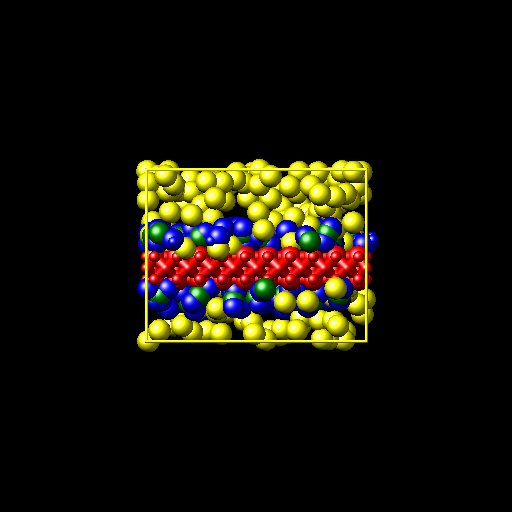
\includegraphics[width=\linewidth,keepaspectratio]{start}
  \caption{}
\end{subfigure}
\begin{subfigure}{0.3\textwidth}
  \centering
  \includegraphics[width=\linewidth,keepaspectratio]{2/2_5000}
  \caption{}
\end{subfigure}
\begin{subfigure}{0.3\textwidth}
  \centering
  \includegraphics[width=\linewidth,keepaspectratio]{2/2_10000}
  \caption{}
\end{subfigure}
\caption{}
\label{fig_1}
\end{figure}

\begin{figure}[H]
\begin{subfigure}{0.24\textwidth}
  \centering
  \includegraphics[width=\linewidth,keepaspectratio]{2/2_mm}
  \caption{mod-mod}
\end{subfigure}
\begin{subfigure}{0.24\textwidth}
  \centering
  \includegraphics[width=\linewidth,keepaspectratio]{2/2_mp}
  \caption{mod-poly}
\end{subfigure}
\begin{subfigure}{0.24\textwidth}
  \centering
  \includegraphics[width=\linewidth,keepaspectratio]{2/2_pp}
  \caption{poly-poly}
\end{subfigure}
\begin{subfigure}{0.24\textwidth}
  \centering
  \includegraphics[width=\linewidth,keepaspectratio]{2/2_ss}
  \caption{soft-soft}
\end{subfigure}
\caption{}
\label{fig_1}
\end{figure}
Increase mod-mod repulsion\newline
Slightly decrease poly-poly attraction


\subsection*{One-three}
pair\_style hybrid/overlay dpd 1 1 34387 \& coul/cut/soft 2 1 5 \& 
lj/cut/soft 2 1 5\newline
pair\_coeff 1 2 coul/cut/soft 0.001\newline
pair\_coeff 3 4 lj/cut/soft 0.05275 10 3 3\newline
pair\_coeff 4 4 lj/cut/soft 0.9     10 3 3\newline
DPD coefficients: $a_{ij}$ and $r_c$
\begin{figure}[H]\begin{tabular}{llll}
MMT           & Head         & Tail         & Polymer      \\
a=500, r=0.95 & a=500, r=0.8 & a=500, r=0.8 & a=500, r=0.8 \\
              & a=100, r=0.8 & a=150, r=0.8 & a=150, r=0.8 \\
              &              & a=150, r=1   & a=150, r=1   \\
              &              &              & a=150, r=1   \\
\end{tabular}\end{figure}

\begin{figure}[H]
\begin{subfigure}{0.3\textwidth}
  \centering
  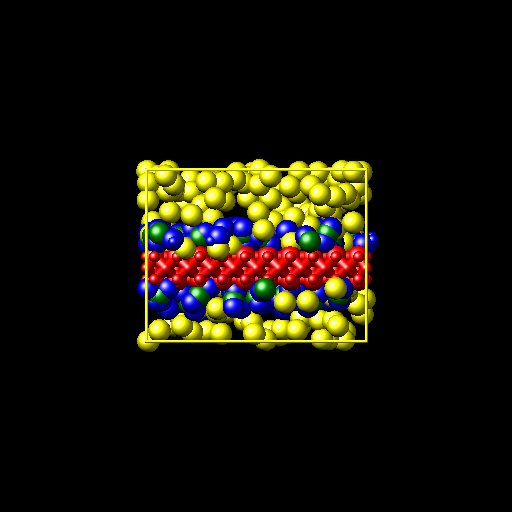
\includegraphics[width=\linewidth,keepaspectratio]{start}
  \caption{}
\end{subfigure}
\begin{subfigure}{0.3\textwidth}
  \centering
  \includegraphics[width=\linewidth,keepaspectratio]{3/3_5000}
  \caption{}
\end{subfigure}
\begin{subfigure}{0.3\textwidth}
  \centering
  \includegraphics[width=\linewidth,keepaspectratio]{3/3_10000}
  \caption{}
\end{subfigure}
\caption{}
\label{fig_1}
\end{figure}

\begin{figure}[H]
\begin{subfigure}{0.24\textwidth}
  \centering
  \includegraphics[width=\linewidth,keepaspectratio]{3/3_mm}
  \caption{mod-mod}
\end{subfigure}
\begin{subfigure}{0.24\textwidth}
  \centering
  \includegraphics[width=\linewidth,keepaspectratio]{3/3_mp}
  \caption{mod-poly}
\end{subfigure}
\begin{subfigure}{0.24\textwidth}
  \centering
  \includegraphics[width=\linewidth,keepaspectratio]{3/3_pp}
  \caption{poly-poly}
\end{subfigure}
\begin{subfigure}{0.24\textwidth}
  \centering
  \includegraphics[width=\linewidth,keepaspectratio]{3/3_ss}
  \caption{soft-soft}
\end{subfigure}
\caption{}
\label{fig_1}
\end{figure}
Slightly increase mod-mod repulsion\newline
Slightly increase mod-poly attraction


\subsection*{One-four}
pair\_style hybrid/overlay dpd 1 1 34387 \& coul/cut/soft 2 1 5 \& 
lj/cut/soft 2 1 5\newline
pair\_coeff 1 2 coul/cut/soft 0.001\newline
pair\_coeff 3 4 lj/cut/soft 0.06    10 3 3\newline
pair\_coeff 4 4 lj/cut/soft 0.9     10 3 3\newline
DPD coefficients: $a_{ij}$ and $r_c$
\begin{figure}[H]\begin{tabular}{llll}
MMT           & Head         & Tail         & Polymer      \\
a=500, r=0.95 & a=500, r=0.8 & a=500, r=0.8 & a=500, r=0.8 \\
              & a=150, r=0.8 & a=150, r=0.8 & a=150, r=0.8 \\
              &              & a=150, r=1   & a=150, r=1   \\
              &              &              & a=150, r=1   \\
\end{tabular}\end{figure}

\begin{figure}[H]
\begin{subfigure}{0.3\textwidth}
  \centering
  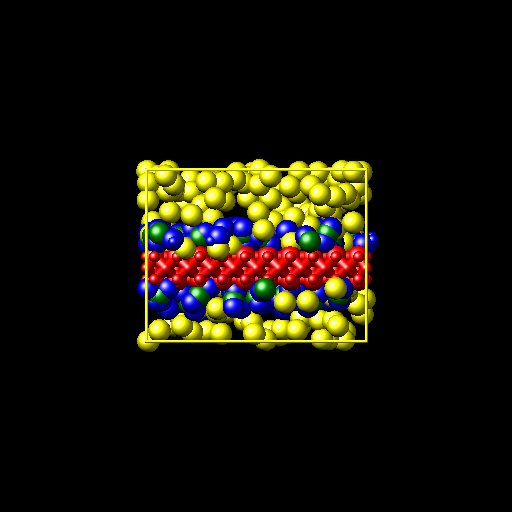
\includegraphics[width=\linewidth,keepaspectratio]{start}
  \caption{}
\end{subfigure}
\begin{subfigure}{0.3\textwidth}
  \centering
  \includegraphics[width=\linewidth,keepaspectratio]{4/4_5000}
  \caption{}
\end{subfigure}
\begin{subfigure}{0.3\textwidth}
  \centering
  \includegraphics[width=\linewidth,keepaspectratio]{4/4_10000}
  \caption{}
\end{subfigure}
\caption{}
\label{fig_1}
\end{figure}

\begin{figure}[H]
\begin{subfigure}{0.24\textwidth}
  \centering
  \includegraphics[width=\linewidth,keepaspectratio]{4/4_mm}
  \caption{mod-mod}
\end{subfigure}
\begin{subfigure}{0.24\textwidth}
  \centering
  \includegraphics[width=\linewidth,keepaspectratio]{4/4_mp}
  \caption{mod-poly}
\end{subfigure}
\begin{subfigure}{0.24\textwidth}
  \centering
  \includegraphics[width=\linewidth,keepaspectratio]{4/4_pp}
  \caption{poly-poly}
\end{subfigure}
\begin{subfigure}{0.24\textwidth}
  \centering
  \includegraphics[width=\linewidth,keepaspectratio]{4/4_ss}
  \caption{soft-soft}
\end{subfigure}
\caption{}
\label{fig_1}
\end{figure}
Increase mod-mod repulsion


\subsection*{One-five}
pair\_style hybrid/overlay dpd 1 1 34387 \& coul/cut/soft 2 1 5 \& 
lj/cut/soft 2 1 5\newline
pair\_coeff 1 2 coul/cut/soft 0.001\newline
pair\_coeff 3 4 lj/cut/soft 0.06    10 3 3\newline
pair\_coeff 4 4 lj/cut/soft 0.9     10 3 3\newline
DPD coefficients: $a_{ij}$ and $r_c$
\begin{figure}[H]\begin{tabular}{llll}
MMT           & Head         & Tail         & Polymer      \\
a=500, r=0.95 & a=500, r=0.8 & a=500, r=0.8 & a=500, r=0.8 \\
              & a=250, r=0.8 & a=250, r=0.8 & a=150, r=0.8 \\
              &              & a=250, r=1   & a=150, r=1   \\
              &              &              & a=150, r=1   \\
\end{tabular}\end{figure}

\begin{figure}[H]
\begin{subfigure}{0.3\textwidth}
  \centering
  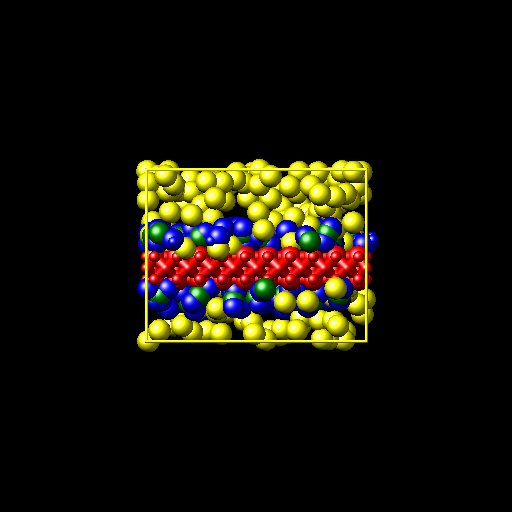
\includegraphics[width=\linewidth,keepaspectratio]{start}
  \caption{}
\end{subfigure}
\begin{subfigure}{0.3\textwidth}
  \centering
  \includegraphics[width=\linewidth,keepaspectratio]{5/5_5000}
  \caption{}
\end{subfigure}
\begin{subfigure}{0.3\textwidth}
  \centering
  \includegraphics[width=\linewidth,keepaspectratio]{5/5_10000}
  \caption{}
\end{subfigure}
\caption{}
\label{fig_1}
\end{figure}

\begin{figure}[H]
\begin{subfigure}{0.24\textwidth}
  \centering
  \includegraphics[width=\linewidth,keepaspectratio]{5/5_mm}
  \caption{mod-mod}
\end{subfigure}
\begin{subfigure}{0.24\textwidth}
  \centering
  \includegraphics[width=\linewidth,keepaspectratio]{5/5_mp}
  \caption{mod-poly}
\end{subfigure}
\begin{subfigure}{0.24\textwidth}
  \centering
  \includegraphics[width=\linewidth,keepaspectratio]{5/5_pp}
  \caption{poly-poly}
\end{subfigure}
\begin{subfigure}{0.24\textwidth}
  \centering
  \includegraphics[width=\linewidth,keepaspectratio]{5/5_ss}
  \caption{soft-soft}
\end{subfigure}
\caption{}
\label{fig_1}
\end{figure}
Sloghtly increase mod-mod repulsion\newline
Sloghtly increase mod-poly repulsion\newline


\subsection*{One-six}
pair\_style hybrid/overlay dpd 1 1 34387 \& coul/cut/soft 2 1 5 \& 
lj/cut/soft 2 1 5\newline
pair\_coeff 1 2 coul/cut/soft 0.001\newline
pair\_coeff 3 4 lj/cut/soft 0.07    10 3 3\newline
pair\_coeff 4 4 lj/cut/soft 0.9     10 3 3\newline
DPD coefficients: $a_{ij}$ and $r_c$
\begin{figure}[H]\begin{tabular}{llll}
MMT           & Head         & Tail         & Polymer      \\
a=500, r=0.95 & a=500, r=0.8 & a=500, r=0.8 & a=500, r=0.8 \\
              & a=350, r=0.8 & a=350, r=0.8 & a=150, r=0.8 \\
              &              & a=350, r=1   & a=150, r=1   \\
              &              &              & a=150, r=1   \\
\end{tabular}\end{figure}

\begin{figure}[H]
\begin{subfigure}{0.3\textwidth}
  \centering
  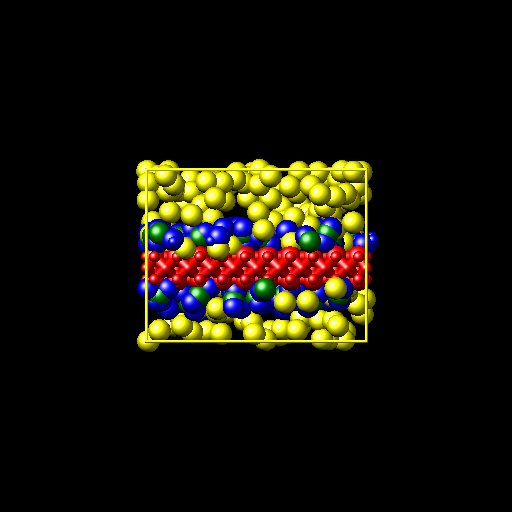
\includegraphics[width=\linewidth,keepaspectratio]{start}
  \caption{}
\end{subfigure}
\begin{subfigure}{0.3\textwidth}
  \centering
  \includegraphics[width=\linewidth,keepaspectratio]{6/6_5000}
  \caption{}
\end{subfigure}
\begin{subfigure}{0.3\textwidth}
  \centering
  \includegraphics[width=\linewidth,keepaspectratio]{6/6_10000}
  \caption{}
\end{subfigure}
\caption{}
\label{fig_1}
\end{figure}

\begin{figure}[H]
\begin{subfigure}{0.24\textwidth}
  \centering
  \includegraphics[width=\linewidth,keepaspectratio]{6/6_mm}
  \caption{mod-mod}
\end{subfigure}
\begin{subfigure}{0.24\textwidth}
  \centering
  \includegraphics[width=\linewidth,keepaspectratio]{6/6_mp}
  \caption{mod-poly}
\end{subfigure}
\begin{subfigure}{0.24\textwidth}
  \centering
  \includegraphics[width=\linewidth,keepaspectratio]{6/6_pp}
  \caption{poly-poly}
\end{subfigure}
\begin{subfigure}{0.24\textwidth}
  \centering
  \includegraphics[width=\linewidth,keepaspectratio]{6/6_ss}
  \caption{soft-soft}
\end{subfigure}
\caption{}
\label{fig_1}
\end{figure}
Sloghtly increase mod-mod repulsion\newline
Sloghtly increase mod-poly repulsion\newline


\subsection*{One-seven}
pair\_style hybrid/overlay dpd 1 1 34387 \& coul/cut/soft 2 1 5 \& 
lj/cut/soft 2 1 5\newline
pair\_coeff 1 2 coul/cut/soft 0.1\newline
pair\_coeff 3 4 lj/cut/soft 0.07    10 3 3\newline
pair\_coeff 4 4 lj/cut/soft 0.9     10 3 3\newline
DPD coefficients: $a_{ij}$ and $r_c$
\begin{figure}[H]\begin{tabular}{llll}
MMT           & Head         & Tail         & Polymer      \\
a=500, r=0.95 & a=500, r=0.8 & a=500, r=0.8 & a=500, r=0.8 \\
              & a=350, r=0.8 & a=350, r=0.8 & a=150, r=0.8 \\
              &              & a=350, r=1   & a=150, r=1   \\
              &              &              & a=150, r=1   \\
\end{tabular}\end{figure}

\begin{figure}[H]
\begin{subfigure}{0.3\textwidth}
  \centering
  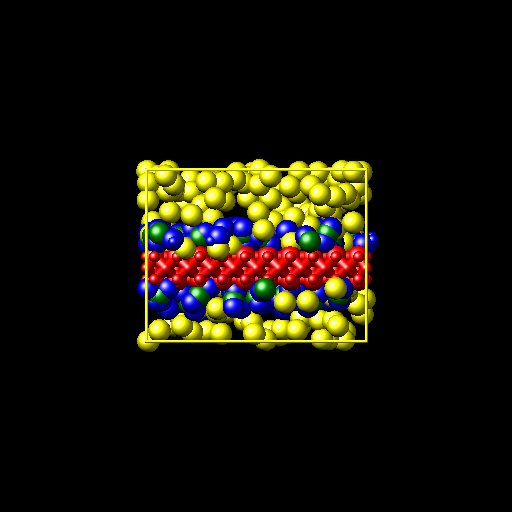
\includegraphics[width=\linewidth,keepaspectratio]{start}
  \caption{}
\end{subfigure}
\begin{subfigure}{0.3\textwidth}
  \centering
  \includegraphics[width=\linewidth,keepaspectratio]{7/7_5000}
  \caption{}
\end{subfigure}
\begin{subfigure}{0.3\textwidth}
  \centering
  \includegraphics[width=\linewidth,keepaspectratio]{7/7_10000}
  \caption{}
\end{subfigure}
\caption{}
\label{fig_1}
\end{figure}

\begin{figure}[H]
\begin{subfigure}{0.24\textwidth}
  \centering
  \includegraphics[width=\linewidth,keepaspectratio]{7/7_mm}
  \caption{mod-mod}
\end{subfigure}
\begin{subfigure}{0.24\textwidth}
  \centering
  \includegraphics[width=\linewidth,keepaspectratio]{7/7_mp}
  \caption{mod-poly}
\end{subfigure}
\begin{subfigure}{0.24\textwidth}
  \centering
  \includegraphics[width=\linewidth,keepaspectratio]{7/7_pp}
  \caption{poly-poly}
\end{subfigure}
\begin{subfigure}{0.24\textwidth}
  \centering
  \includegraphics[width=\linewidth,keepaspectratio]{7/7_ss}
  \caption{soft-soft}
\end{subfigure}
\caption{}
\label{fig_1}
\end{figure}
Sloghtly increase mod-mod repulsion\newline
Sloghtly increase mod-poly repulsion


\subsection*{One-eight}
pair\_style hybrid/overlay dpd 1 1 34387 \& coul/cut/soft 2 1 5 \& 
lj/cut/soft 2 1 5\newline
pair\_coeff 1 2 coul/cut/soft 0.1\newline
pair\_coeff 3 4 lj/cut/soft 0.07    10 3 3\newline
pair\_coeff 4 4 lj/cut/soft 0.9     10 3 3\newline
DPD coefficients: $a_{ij}$ and $r_c$
\begin{figure}[H]\begin{tabular}{llll}
MMT           & Head         & Tail         & Polymer      \\
a=500, r=0.95 & a=500, r=0.8 & a=500, r=0.8 & a=500, r=0.8 \\
              & a=150, r=0.8 & a=150, r=0.8 & a=150, r=0.8 \\
              &              & a=150, r=1   & a=150, r=1   \\
              &              &              & a=150, r=1   \\
\end{tabular}\end{figure}

\begin{figure}[H]
\begin{subfigure}{0.3\textwidth}
  \centering
  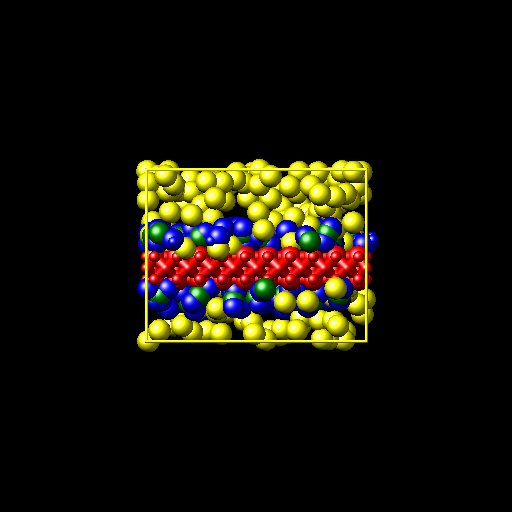
\includegraphics[width=\linewidth,keepaspectratio]{start}
  \caption{}
\end{subfigure}
\begin{subfigure}{0.3\textwidth}
  \centering
  \includegraphics[width=\linewidth,keepaspectratio]{8/8_5000}
  \caption{}
\end{subfigure}
\begin{subfigure}{0.3\textwidth}
  \centering
  \includegraphics[width=\linewidth,keepaspectratio]{8/8_10000}
  \caption{}
\end{subfigure}
\caption{}
\label{fig_1}
\end{figure}

\begin{figure}[H]
\begin{subfigure}{0.24\textwidth}
  \centering
  \includegraphics[width=\linewidth,keepaspectratio]{8/8_mm}
  \caption{mod-mod}
\end{subfigure}
\begin{subfigure}{0.24\textwidth}
  \centering
  \includegraphics[width=\linewidth,keepaspectratio]{8/8_mp}
  \caption{mod-poly}
\end{subfigure}
\begin{subfigure}{0.24\textwidth}
  \centering
  \includegraphics[width=\linewidth,keepaspectratio]{8/8_pp}
  \caption{poly-poly}
\end{subfigure}
\begin{subfigure}{0.24\textwidth}
  \centering
  \includegraphics[width=\linewidth,keepaspectratio]{8/8_ss}
  \caption{soft-soft}
\end{subfigure}
\caption{}
\label{fig_1}
\end{figure}
Decrease mod-mod repulsion\newline
Decrease poly-poly attraction


\subsection*{One-nine}
pair\_style hybrid/overlay dpd 1 1 34387 \& coul/cut/soft 2 1 5 \& 
lj/cut/soft 2 1 5\newline
pair\_coeff 1 2 coul/cut/soft 0.1\newline
pair\_coeff 3 4 lj/cut/soft 0.07    10 3 3\newline
pair\_coeff 4 4 lj/cut/soft 0.8     10 3 3\newline
DPD coefficients: $a_{ij}$ and $r_c$
\begin{figure}[H]\begin{tabular}{llll}
MMT           & Head         & Tail         & Polymer      \\
a=500, r=0.95 & a=500, r=0.8 & a=500, r=0.8 & a=500, r=0.8 \\
              & a=75,  r=0.8 & a=75,  r=0.8 & a=150, r=0.8 \\
              &              & a=75,  r=1   & a=150, r=1   \\
              &              &              & a=150, r=1   \\
\end{tabular}\end{figure}

\begin{figure}[H]
\begin{subfigure}{0.3\textwidth}
  \centering
  \includegraphics[width=\linewidth,keepaspectratio]{start}
  \caption{}
\end{subfigure}
\begin{subfigure}{0.3\textwidth}
  \centering
  \includegraphics[width=\linewidth,keepaspectratio]{9/9_5000}
  \caption{}
\end{subfigure}
\begin{subfigure}{0.3\textwidth}
  \centering
  \includegraphics[width=\linewidth,keepaspectratio]{9/9_10000}
  \caption{}
\end{subfigure}
\caption{}
\label{fig_1}
\end{figure}

\begin{figure}[H]
\begin{subfigure}{0.24\textwidth}
  \centering
  \includegraphics[width=\linewidth,keepaspectratio]{9/9_mm}
  \caption{mod-mod}
\end{subfigure}
\begin{subfigure}{0.24\textwidth}
  \centering
  \includegraphics[width=\linewidth,keepaspectratio]{9/9_mp}
  \caption{mod-poly}
\end{subfigure}
\begin{subfigure}{0.24\textwidth}
  \centering
  \includegraphics[width=\linewidth,keepaspectratio]{9/9_pp}
  \caption{poly-poly}
\end{subfigure}
\begin{subfigure}{0.24\textwidth}
  \centering
  \includegraphics[width=\linewidth,keepaspectratio]{9/9_ss}
  \caption{soft-soft}
\end{subfigure}
\caption{}
\label{fig_1}
\end{figure}
Slightly decrease mod-mod repulsion\newline
Increase poly-poly attraction



\subsection*{One-ten}
pair\_style hybrid/overlay dpd 1 1 34387 \& coul/cut/soft 2 1 5 \& 
lj/cut/soft 2 1 5\newline
pair\_coeff 1 2 coul/cut/soft 0.1\newline
pair\_coeff 3 4 lj/cut/soft 0.07    10 3 3\newline
pair\_coeff 4 4 lj/cut/soft 0.85    10 3 3\newline
DPD coefficients: $a_{ij}$ and $r_c$
\begin{figure}[H]\begin{tabular}{llll}
MMT           & Head         & Tail         & Polymer      \\
a=500, r=0.95 & a=500, r=0.8 & a=500, r=0.8 & a=500, r=0.8 \\
              & a=50,  r=0.8 & a=50,  r=0.8 & a=150, r=0.8 \\
              &              & a=50,  r=1   & a=150, r=1   \\
              &              &              & a=150, r=1   \\
\end{tabular}\end{figure}

\begin{figure}[H]
\begin{subfigure}{0.3\textwidth}
  \centering
  \includegraphics[width=\linewidth,keepaspectratio]{start}
  \caption{}
\end{subfigure}
\begin{subfigure}{0.3\textwidth}
  \centering
  \includegraphics[width=\linewidth,keepaspectratio]{10/10_5000}
  \caption{}
\end{subfigure}
\begin{subfigure}{0.3\textwidth}
  \centering
  \includegraphics[width=\linewidth,keepaspectratio]{10/10_10000}
  \caption{}
\end{subfigure}
\caption{}
\label{fig_1}
\end{figure}

\begin{figure}[H]
\begin{subfigure}{0.24\textwidth}
  \centering
  \includegraphics[width=\linewidth,keepaspectratio]{10/10_mm}
  \caption{mod-mod}
\end{subfigure}
\begin{subfigure}{0.24\textwidth}
  \centering
  \includegraphics[width=\linewidth,keepaspectratio]{10/10_mp}
  \caption{mod-poly}
\end{subfigure}
\begin{subfigure}{0.24\textwidth}
  \centering
  \includegraphics[width=\linewidth,keepaspectratio]{10/10_pp}
  \caption{poly-poly}
\end{subfigure}
\begin{subfigure}{0.24\textwidth}
  \centering
  \includegraphics[width=\linewidth,keepaspectratio]{10/10_ss}
  \caption{soft-soft}
\end{subfigure}
\caption{}
\label{fig_1}
\end{figure}
Slightly decrease mod-mod repulsion\newline
Slightly increase poly-poly attraction



\subsection*{One-eleven}
pair\_style hybrid/overlay dpd 1 1 34387 \& coul/cut/soft 2 1 5 \& 
lj/cut/soft 2 1 5\newline
pair\_coeff 1 2 coul/cut/soft 0.1\newline
pair\_coeff 3 4 lj/cut/soft 0.07    10 3 3\newline
pair\_coeff 4 4 lj/cut/soft 0.875    10 3 3\newline
DPD coefficients: $a_{ij}$ and $r_c$
\begin{figure}[H]\begin{tabular}{llll}
MMT           & Head         & Tail         & Polymer      \\
a=500, r=0.95 & a=500, r=0.8 & a=500, r=0.8 & a=500, r=0.8 \\
              & a=40,  r=0.8 & a=40,  r=0.8 & a=150, r=0.8 \\
              &              & a=40,  r=1   & a=150, r=1   \\
              &              &              & a=150, r=1   \\
\end{tabular}\end{figure}

\begin{figure}[H]
\begin{subfigure}{0.3\textwidth}
  \centering
  \includegraphics[width=\linewidth,keepaspectratio]{start}
  \caption{}
\end{subfigure}
\begin{subfigure}{0.3\textwidth}
  \centering
  \includegraphics[width=\linewidth,keepaspectratio]{11/11_5000}
  \caption{}
\end{subfigure}
\begin{subfigure}{0.3\textwidth}
  \centering
  \includegraphics[width=\linewidth,keepaspectratio]{11/11_10000}
  \caption{}
\end{subfigure}
\caption{}
\label{fig_1}
\end{figure}

\begin{figure}[H]
\begin{subfigure}{0.24\textwidth}
  \centering
  \includegraphics[width=\linewidth,keepaspectratio]{11/11_mm}
  \caption{mod-mod}
\end{subfigure}
\begin{subfigure}{0.24\textwidth}
  \centering
  \includegraphics[width=\linewidth,keepaspectratio]{11/11_mp}
  \caption{mod-poly}
\end{subfigure}
\begin{subfigure}{0.24\textwidth}
  \centering
  \includegraphics[width=\linewidth,keepaspectratio]{11/11_pp}
  \caption{poly-poly}
\end{subfigure}
\begin{subfigure}{0.24\textwidth}
  \centering
  \includegraphics[width=\linewidth,keepaspectratio]{11/11_ss}
  \caption{soft-soft}
\end{subfigure}
\caption{}
\label{fig_1}
\end{figure}
Slightly decrease mod-mod repulsion\newline
Slightly increase poly-poly attraction



\subsection*{One-12}
pair\_style hybrid/overlay dpd 1 1 34387 \& coul/cut/soft 2 1 5 \& 
lj/cut/soft 2 1 5\newline
pair\_coeff 1 1 coul/cut/soft 0.25
pair\_coeff 1 2 coul/cut/soft 0.5\newline
pair\_coeff 3 4 lj/cut/soft 0.07    10 3 3\newline
pair\_coeff 4 4 lj/cut/soft 0.875    10 3 3\newline
DPD coefficients: $a_{ij}$ and $r_c$
\begin{figure}[H]\begin{tabular}{llll}
MMT             & Head         & Tail         & Polymer      \\
a=50000, r=0.95 & a=500, r=0.8 & a=500, r=0.8 & a=500, r=0.8 \\
                & a=40,  r=0.8 & a=40,  r=0.8 & a=150, r=0.8 \\
                &              & a=40,  r=1   & a=150, r=1   \\
                &              &              & a=150, r=1   \\
\end{tabular}\end{figure}

\begin{figure}[H]
\begin{subfigure}{0.3\textwidth}
  \centering
  \includegraphics[width=\linewidth,keepaspectratio]{start}
  \caption{}
\end{subfigure}
\begin{subfigure}{0.3\textwidth}
  \centering
  \includegraphics[width=\linewidth,keepaspectratio]{12/12_5000}
  \caption{}
\end{subfigure}
\begin{subfigure}{0.3\textwidth}
  \centering
  \includegraphics[width=\linewidth,keepaspectratio]{12/12_10000}
  \caption{}
\end{subfigure}
\caption{}
\label{fig_1}
\end{figure}

\begin{figure}[H]
\begin{subfigure}{0.24\textwidth}
  \centering
  \includegraphics[width=\linewidth,keepaspectratio]{12/12_mm}
  \caption{mod-mod}
\end{subfigure}
\begin{subfigure}{0.24\textwidth}
  \centering
  \includegraphics[width=\linewidth,keepaspectratio]{12/12_mp}
  \caption{mod-poly}
\end{subfigure}
\begin{subfigure}{0.24\textwidth}
  \centering
  \includegraphics[width=\linewidth,keepaspectratio]{12/12_pp}
  \caption{poly-poly}
\end{subfigure}
\begin{subfigure}{0.24\textwidth}
  \centering
  \includegraphics[width=\linewidth,keepaspectratio]{12/12_ss}
  \caption{soft-soft}
\end{subfigure}
\caption{}
\label{fig_1}
\end{figure}




\subsection*{One-13}
pair\_style hybrid/overlay dpd 1 1 34387 \& coul/cut/soft 2 1 5 \& 
lj/cut/soft 2 1 5\newline
pair\_coeff 1 1 coul/cut/soft 0.25
pair\_coeff 1 2 coul/cut/soft 0.5\newline
pair\_coeff 3 4 lj/cut/soft 0.07    10 3 3\newline
pair\_coeff 4 4 lj/cut/soft 0.85    10 3 3\newline
DPD coefficients: $a_{ij}$ and $r_c$
\begin{figure}[H]\begin{tabular}{llll}
MMT             & Head         & Tail         & Polymer      \\
a=50000, r=0.95 & a=500, r=0.8 & a=500, r=0.8 & a=500, r=0.8 \\
                & a=100, r=0.8 & a=100, r=0.8 & a=150, r=0.8 \\
                &              & a=40,  r=1   & a=250, r=1   \\
                &              &              & a=250, r=1   \\
\end{tabular}\end{figure}

\begin{figure}[H]
\begin{subfigure}{0.3\textwidth}
  \centering
  \includegraphics[width=\linewidth,keepaspectratio]{start}
  \caption{}
\end{subfigure}
\begin{subfigure}{0.3\textwidth}
  \centering
  \includegraphics[width=\linewidth,keepaspectratio]{13/13_5000}
  \caption{}
\end{subfigure}
\begin{subfigure}{0.3\textwidth}
  \centering
  \includegraphics[width=\linewidth,keepaspectratio]{13/13_10000}
  \caption{}
\end{subfigure}
\caption{}
\label{fig_1}
\end{figure}

\begin{figure}[H]
\begin{subfigure}{0.24\textwidth}
  \centering
  \includegraphics[width=\linewidth,keepaspectratio]{13/13_mm}
  \caption{mod-mod}
\end{subfigure}
\begin{subfigure}{0.24\textwidth}
  \centering
  \includegraphics[width=\linewidth,keepaspectratio]{13/13_mp}
  \caption{mod-poly}
\end{subfigure}
\begin{subfigure}{0.24\textwidth}
  \centering
  \includegraphics[width=\linewidth,keepaspectratio]{13/13_pp}
  \caption{poly-poly}
\end{subfigure}
\begin{subfigure}{0.24\textwidth}
  \centering
  \includegraphics[width=\linewidth,keepaspectratio]{13/13_ss}
  \caption{soft-soft}
\end{subfigure}
\caption{}
\label{fig_1}
\end{figure}




\subsection*{One-14}
pair\_style hybrid/overlay dpd 1 1 34387 \& coul/cut/soft 2 1 5 \& 
lj/cut/soft 2 1 5\newline
pair\_coeff 1 1 coul/cut/soft 0.25
pair\_coeff 1 2 coul/cut/soft 0.5\newline
pair\_coeff 3 4 lj/cut/soft 0.07    10 3 3\newline
pair\_coeff 4 4 lj/cut/soft 0.85    10 3 3\newline
DPD coefficients: $a_{ij}$ and $r_c$
\begin{figure}[H]\begin{tabular}{llll}
MMT             & Head         & Tail         & Polymer      \\
a=50000, r=0.95 & a=500, r=0.8 & a=500, r=0.8 & a=500, r=0.8 \\
                & a=75,  r=0.8 & a=75,  r=0.8 & a=150, r=0.8 \\
                &              & a=75,  r=1   & a=250, r=1   \\
                &              &              & a=500, r=1   \\
\end{tabular}\end{figure}

\begin{figure}[H]
\begin{subfigure}{0.3\textwidth}
  \centering
  \includegraphics[width=\linewidth,keepaspectratio]{start}
  \caption{}
\end{subfigure}
\begin{subfigure}{0.3\textwidth}
  \centering
  \includegraphics[width=\linewidth,keepaspectratio]{14/14_5000}
  \caption{}
\end{subfigure}
\begin{subfigure}{0.3\textwidth}
  \centering
  \includegraphics[width=\linewidth,keepaspectratio]{14/14_10000}
  \caption{}
\end{subfigure}
\caption{}
\label{fig_1}
\end{figure}

\begin{figure}[H]
\begin{subfigure}{0.24\textwidth}
  \centering
  \includegraphics[width=\linewidth,keepaspectratio]{14/14_mm}
  \caption{mod-mod}
\end{subfigure}
\begin{subfigure}{0.24\textwidth}
  \centering
  \includegraphics[width=\linewidth,keepaspectratio]{14/14_mp}
  \caption{mod-poly}
\end{subfigure}
\begin{subfigure}{0.24\textwidth}
  \centering
  \includegraphics[width=\linewidth,keepaspectratio]{14/14_pp}
  \caption{poly-poly}
\end{subfigure}
\begin{subfigure}{0.24\textwidth}
  \centering
  \includegraphics[width=\linewidth,keepaspectratio]{14/14_ss}
  \caption{soft-soft}
\end{subfigure}
\caption{}
\label{fig_1}
\end{figure}



\subsection*{One-15}
pair\_style hybrid/overlay dpd 1 1 34387 \& coul/cut/soft 2 1 5 \& 
lj/cut/soft 2 1 5\newline
pair\_coeff 1 1 coul/cut/soft 0.25
pair\_coeff 1 2 coul/cut/soft 0.5\newline
pair\_coeff 3 4 lj/cut/soft 0.07    10 3 3\newline
pair\_coeff 4 4 lj/cut/soft 0.85    10 3 3\newline
DPD coefficients: $a_{ij}$ and $r_c$
\begin{figure}[H]\begin{tabular}{llll}
MMT             & Head         & Tail         & Polymer      \\
a=50000, r=0.95 & a=500, r=0.8 & a=500, r=0.8 & a=500, r=0.8 \\
                & a=50,  r=0.8 & a=50,  r=0.8 & a=150, r=0.8 \\
                &              & a=50,  r=1   & a=350, r=1   \\
                &              &              & a=400, r=1   \\
\end{tabular}\end{figure}

\begin{figure}[H]
\begin{subfigure}{0.3\textwidth}
  \centering
  \includegraphics[width=\linewidth,keepaspectratio]{start}
  \caption{}
\end{subfigure}
\begin{subfigure}{0.3\textwidth}
  \centering
  \includegraphics[width=\linewidth,keepaspectratio]{15/15_5000}
  \caption{}
\end{subfigure}
\begin{subfigure}{0.3\textwidth}
  \centering
  \includegraphics[width=\linewidth,keepaspectratio]{15/15_10000}
  \caption{}
\end{subfigure}
\caption{}
\label{fig_1}
\end{figure}

\begin{figure}[H]
\begin{subfigure}{0.24\textwidth}
  \centering
  \includegraphics[width=\linewidth,keepaspectratio]{15/15_mm}
  \caption{mod-mod}
\end{subfigure}
\begin{subfigure}{0.24\textwidth}
  \centering
  \includegraphics[width=\linewidth,keepaspectratio]{15/15_mp}
  \caption{mod-poly}
\end{subfigure}
\begin{subfigure}{0.24\textwidth}
  \centering
  \includegraphics[width=\linewidth,keepaspectratio]{15/15_pp}
  \caption{poly-poly}
\end{subfigure}
\begin{subfigure}{0.24\textwidth}
  \centering
  \includegraphics[width=\linewidth,keepaspectratio]{15/15_ss}
  \caption{soft-soft}
\end{subfigure}
\caption{}
\label{fig_1}
\end{figure}


\subsection*{One-16}
pair\_style hybrid/overlay dpd 1 1 34387 \& coul/cut/soft 2 1 5 \& 
lj/cut/soft 2 1 5\newline
pair\_coeff 1 1 coul/cut/soft 0.25
pair\_coeff 1 2 coul/cut/soft 0.5\newline
pair\_coeff 3 4 lj/cut/soft 0.07    10 3 3\newline
pair\_coeff 4 4 lj/cut/soft 0.85    10 3 3\newline
DPD coefficients: $a_{ij}$ and $r_c$
\begin{figure}[H]\begin{tabular}{llll}
MMT             & Head         & Tail         & Polymer      \\
a=50000, r=0.95 & a=500, r=0.8 & a=500, r=0.8 & a=500, r=0.8 \\
                & a=40,  r=0.8 & a=40,  r=0.8 & a=300, r=0.8 \\
                &              & a=40,  r=1   & a=300, r=1   \\
                &              &              & a=450, r=1   \\
\end{tabular}\end{figure}

\begin{figure}[H]
\begin{subfigure}{0.3\textwidth}
  \centering
  \includegraphics[width=\linewidth,keepaspectratio]{start}
  \caption{}
\end{subfigure}
\begin{subfigure}{0.3\textwidth}
  \centering
  \includegraphics[width=\linewidth,keepaspectratio]{16/16_5000}
  \caption{}
\end{subfigure}
\begin{subfigure}{0.3\textwidth}
  \centering
  \includegraphics[width=\linewidth,keepaspectratio]{16/16_10000}
  \caption{}
\end{subfigure}
\caption{}
\label{fig_1}
\end{figure}

\begin{figure}[H]
\begin{subfigure}{0.24\textwidth}
  \centering
  \includegraphics[width=\linewidth,keepaspectratio]{16/16_mm}
  \caption{mod-mod}
\end{subfigure}
\begin{subfigure}{0.24\textwidth}
  \centering
  \includegraphics[width=\linewidth,keepaspectratio]{16/16_mp}
  \caption{mod-poly}
\end{subfigure}
\begin{subfigure}{0.24\textwidth}
  \centering
  \includegraphics[width=\linewidth,keepaspectratio]{16/16_pp}
  \caption{poly-poly}
\end{subfigure}
\begin{subfigure}{0.24\textwidth}
  \centering
  \includegraphics[width=\linewidth,keepaspectratio]{16/16_ss}
  \caption{soft-soft}
\end{subfigure}
\caption{}
\label{fig_1}
\end{figure}


\subsection*{One-17 (==18?)}
pair\_style hybrid/overlay dpd 1 1 34387 \& coul/cut/soft 2 1 5 \& 
lj/cut/soft 2 1 5\newline
pair\_coeff 1 1 coul/cut/soft 0.25
pair\_coeff 1 2 coul/cut/soft 0.5\newline
pair\_coeff 3 4 lj/cut/soft 0.07    10 3 3\newline
pair\_coeff 4 4 lj/cut/soft 0.85    10 3 3\newline
DPD coefficients: $a_{ij}$ and $r_c$
\begin{figure}[H]\begin{tabular}{llll}
MMT             & Head         & Tail         & Polymer      \\
a=50000, r=0.95 & a=500, r=0.8 & a=500, r=0.8 & a=500, r=0.8 \\
                & a=35,  r=0.8 & a=35,  r=0.8 & a=300, r=0.8 \\
                &              & a=35,  r=1   & a=300, r=1   \\
                &              &              & a=600, r=1   \\
\end{tabular}\end{figure}

\begin{figure}[H]
\begin{subfigure}{0.3\textwidth}
  \centering
  \includegraphics[width=\linewidth,keepaspectratio]{start}
  \caption{}
\end{subfigure}
\begin{subfigure}{0.3\textwidth}
  \centering
  \includegraphics[width=\linewidth,keepaspectratio]{17/17_5000}
  \caption{5k}
\end{subfigure}
\begin{subfigure}{0.3\textwidth}
  \centering
  \includegraphics[width=\linewidth,keepaspectratio]{17/17_10000}
  \caption{10k}
\end{subfigure}
\caption{}
\label{fig_1}
\end{figure}

\begin{figure}[H]
\begin{subfigure}{0.24\textwidth}
  \centering
  \includegraphics[width=\linewidth,keepaspectratio]{17/17_mm}
  \caption{mod-mod}
\end{subfigure}
\begin{subfigure}{0.24\textwidth}
  \centering
  \includegraphics[width=\linewidth,keepaspectratio]{17/17_mp}
  \caption{mod-poly}
\end{subfigure}
\begin{subfigure}{0.24\textwidth}
  \centering
  \includegraphics[width=\linewidth,keepaspectratio]{17/17_pp}
  \caption{poly-poly}
\end{subfigure}
\begin{subfigure}{0.24\textwidth}
  \centering
  \includegraphics[width=\linewidth,keepaspectratio]{17/17_ss}
  \caption{soft-soft}
\end{subfigure}
\caption{}
\label{fig_1}
\end{figure}




\subsection*{One-18}
pair\_style hybrid/overlay dpd 1 1 34387 \& coul/cut/soft 2 1 5 \& 
lj/cut/soft 2 1 5\newline
pair\_coeff 1 1 coul/cut/soft 0.25
pair\_coeff 1 2 coul/cut/soft 0.5\newline
pair\_coeff 3 4 lj/cut/soft 0.07    10 3 3\newline
pair\_coeff 4 4 lj/cut/soft 0.85    10 3 3\newline
DPD coefficients: $a_{ij}$ and $r_c$
\begin{figure}[H]\begin{tabular}{llll}
MMT             & Head         & Tail         & Polymer      \\
a=50000, r=0.95 & a=500, r=0.8 & a=500, r=0.8 & a=500, r=0.8 \\
                & a=35,  r=0.8 & a=35,  r=0.8 & a=300, r=0.8 \\
                &              & a=35,  r=1   & a=300, r=1   \\
                &              &              & a=600, r=1   \\
\end{tabular}\end{figure}

\begin{figure}[H]
\begin{subfigure}{0.3\textwidth}
  \centering
  \includegraphics[width=\linewidth,keepaspectratio]{start}
  \caption{}
\end{subfigure}
\begin{subfigure}{0.3\textwidth}
  \centering
  \includegraphics[width=\linewidth,keepaspectratio]{18/18_10000}
  \caption{10k}
\end{subfigure}
\begin{subfigure}{0.3\textwidth}
  \centering
  \includegraphics[width=\linewidth,keepaspectratio]{18/18_25000}
  \caption{25k}
\end{subfigure}
\caption{}
\label{fig_1}
\end{figure}

\begin{figure}[H]
\begin{subfigure}{0.24\textwidth}
  \centering
  \includegraphics[width=\linewidth,keepaspectratio]{18/18_mm}
  \caption{mod-mod}
\end{subfigure}
\begin{subfigure}{0.24\textwidth}
  \centering
  \includegraphics[width=\linewidth,keepaspectratio]{18/18_mp}
  \caption{mod-poly}
\end{subfigure}
\begin{subfigure}{0.24\textwidth}
  \centering
  \includegraphics[width=\linewidth,keepaspectratio]{18/18_pp}
  \caption{poly-poly}
\end{subfigure}
\begin{subfigure}{0.24\textwidth}
  \centering
  \includegraphics[width=\linewidth,keepaspectratio]{18/18_ss}
  \caption{soft-soft}
\end{subfigure}
\caption{}
\label{fig_1}
\end{figure}




\subsection*{One-19}
pair\_style hybrid/overlay dpd 1 1 34387 \& coul/cut/soft 2 1 5 \& 
lj/cut/soft 2 1 5\newline
pair\_coeff 1 1 coul/cut/soft 0.25
pair\_coeff 1 2 coul/cut/soft 0.5\newline
pair\_coeff 3 4 lj/cut/soft 0.07    10 3 3\newline
pair\_coeff 4 4 lj/cut/soft 0.85    10 3 3\newline
DPD coefficients: $a_{ij}$ and $r_c$
\begin{figure}[H]\begin{tabular}{llll}
MMT             & Head         & Tail         & Polymer      \\
a=50000, r=0.95 & a=500, r=0.8 & a=500, r=0.8 & a=500, r=0.8 \\
                & a=40,  r=0.8 & a=40,  r=0.8 & a=300, r=0.8 \\
                &              & a=40,  r=1   & a=250, r=1   \\
                &              &              & a=800, r=1   \\
\end{tabular}\end{figure}

\begin{figure}[H]
\begin{subfigure}{0.3\textwidth}
  \centering
  \includegraphics[width=\linewidth,keepaspectratio]{start}
  \caption{}
\end{subfigure}
\begin{subfigure}{0.3\textwidth}
  \centering
  \includegraphics[width=\linewidth,keepaspectratio]{19/19_10000}
  \caption{10k}
\end{subfigure}
\begin{subfigure}{0.3\textwidth}
  \centering
  \includegraphics[width=\linewidth,keepaspectratio]{19/19_25000}
  \caption{25k}
\end{subfigure}
\caption{}
\label{fig_1}
\end{figure}

\begin{figure}[H]
\begin{subfigure}{0.24\textwidth}
  \centering
  \includegraphics[width=\linewidth,keepaspectratio]{19/19_mm}
  \caption{mod-mod}
\end{subfigure}
\begin{subfigure}{0.24\textwidth}
  \centering
  \includegraphics[width=\linewidth,keepaspectratio]{19/19_mp}
  \caption{mod-poly}
\end{subfigure}
\begin{subfigure}{0.24\textwidth}
  \centering
  \includegraphics[width=\linewidth,keepaspectratio]{19/19_pp}
  \caption{poly-poly}
\end{subfigure}
\begin{subfigure}{0.24\textwidth}
  \centering
  \includegraphics[width=\linewidth,keepaspectratio]{19/19_ss}
  \caption{soft-soft}
\end{subfigure}
\caption{}
\label{fig_1}
\end{figure}



\subsection*{One-20}
pair\_style hybrid/overlay dpd 1 1 34387 \& coul/cut/soft 2 1 5 \& 
lj/cut/soft 2 1 5\newline
pair\_coeff 1 1 coul/cut/soft 0.25
pair\_coeff 1 2 coul/cut/soft 0.5\newline
pair\_coeff 3 4 lj/cut/soft 0.07    10 3 3\newline
pair\_coeff 4 4 lj/cut/soft 0.85    10 3 3\newline
DPD coefficients: $a_{ij}$ and $r_c$
\begin{figure}[H]\begin{tabular}{llll}
MMT             & Head         & Tail         & Polymer      \\
a=50000, r=0.95 & a=500, r=0.8 & a=500, r=0.8 & a=500, r=0.8 \\
                & a=25,  r=0.8 & a=25,  r=0.8 & a=300, r=0.8 \\
                &              & a=25,  r=1   & a=250, r=1   \\
                &              &              & a=800, r=1   \\
\end{tabular}\end{figure}

\begin{figure}[H]
\begin{subfigure}{0.3\textwidth}
  \centering
  \includegraphics[width=\linewidth,keepaspectratio]{start}
  \caption{}
\end{subfigure}
\begin{subfigure}{0.3\textwidth}
  \centering
  \includegraphics[width=\linewidth,keepaspectratio]{20/20_10000}
  \caption{10k}
\end{subfigure}
\begin{subfigure}{0.3\textwidth}
  \centering
  \includegraphics[width=\linewidth,keepaspectratio]{20/20_25000}
  \caption{25k}
\end{subfigure}
\caption{}
\label{fig_1}
\end{figure}

\begin{figure}[H]
\begin{subfigure}{0.24\textwidth}
  \centering
  \includegraphics[width=\linewidth,keepaspectratio]{20/20_mm}
  \caption{mod-mod}
\end{subfigure}
\begin{subfigure}{0.24\textwidth}
  \centering
  \includegraphics[width=\linewidth,keepaspectratio]{20/20_mp}
  \caption{mod-poly}
\end{subfigure}
\begin{subfigure}{0.24\textwidth}
  \centering
  \includegraphics[width=\linewidth,keepaspectratio]{20/20_pp}
  \caption{poly-poly}
\end{subfigure}
\begin{subfigure}{0.24\textwidth}
  \centering
  \includegraphics[width=\linewidth,keepaspectratio]{20/20_ss}
  \caption{soft-soft}
\end{subfigure}
\caption{}
\label{fig_1}
\end{figure}


\section*{NVT}


\subsection*{One-21}
pair\_style hybrid/overlay dpd 1 1 34387 \& coul/cut/soft 2 1 5 \& 
lj/cut/soft 2 1 5\newline
pair\_coeff 1 1 coul/cut/soft 0.25
pair\_coeff 1 2 coul/cut/soft 0.5\newline
pair\_coeff 3 4 lj/cut/soft 0.07    10 3 3\newline
pair\_coeff 4 4 lj/cut/soft 0.85    10 3 3\newline
DPD coefficients: $a_{ij}$ and $r_c$
\begin{figure}[H]\begin{tabular}{llll}
MMT             & Head         & Tail         & Polymer      \\
a=50000, r=0.95 & a=500, r=0.8 & a=500, r=0.8 & a=500, r=0.8 \\
                & a=25,  r=0.8 & a=25,  r=0.8 & a=300, r=0.8 \\
                &              & a=25,  r=1   & a=250, r=1   \\
                &              &              & a=800, r=1   \\
\end{tabular}\end{figure}

\begin{figure}[H]
\begin{subfigure}{0.3\textwidth}
  \centering
  \includegraphics[width=\linewidth,keepaspectratio]{start}
  \caption{}
\end{subfigure}
\begin{subfigure}{0.3\textwidth}
  \centering
  \includegraphics[width=\linewidth,keepaspectratio]{21/21_10000}
  \caption{10k}
\end{subfigure}
\begin{subfigure}{0.3\textwidth}
  \centering
  \includegraphics[width=\linewidth,keepaspectratio]{21/21_25000}
  \caption{25k}
\end{subfigure}
\caption{}
\label{fig_1}
\end{figure}

\begin{figure}[H]
\begin{subfigure}{0.24\textwidth}
  \centering
  \includegraphics[width=\linewidth,keepaspectratio]{21/21_mm}
  \caption{mod-mod}
\end{subfigure}
\begin{subfigure}{0.24\textwidth}
  \centering
  \includegraphics[width=\linewidth,keepaspectratio]{21/21_mp}
  \caption{mod-poly}
\end{subfigure}
\begin{subfigure}{0.24\textwidth}
  \centering
  \includegraphics[width=\linewidth,keepaspectratio]{21/21_pp}
  \caption{poly-poly}
\end{subfigure}
\begin{subfigure}{0.24\textwidth}
  \centering
  \includegraphics[width=\linewidth,keepaspectratio]{21/21_ss}
  \caption{soft-soft}
\end{subfigure}
\caption{}
\label{fig_1}
\end{figure}




\subsection*{One-22}
pair\_style hybrid/overlay dpd 1 1 34387 \& coul/cut/soft 2 1 5 \& 
lj/cut/soft 2 1 5\newline
pair\_coeff 1 1 coul/cut/soft 0.25
pair\_coeff 1 2 coul/cut/soft 0.5\newline
pair\_coeff 3 4 lj/cut/soft 0.07    10 3 3\newline
pair\_coeff 4 4 lj/cut/soft 0.85    10 3 3\newline
DPD coefficients: $a_{ij}$ and $r_c$
\begin{figure}[H]\begin{tabular}{llll}
MMT             & Head         & Tail         & Polymer      \\
a=50000, r=0.95 & a=500, r=0.8 & a=500, r=0.8 & a=500, r=0.8 \\
                & a=25,  r=0.8 & a=25,  r=0.8 & a=200, r=0.8 \\
                &              & a=25,  r=1   & a=200, r=1   \\
                &              &              & a=200, r=1   \\
\end{tabular}\end{figure}

\begin{figure}[H]
\begin{subfigure}{0.3\textwidth}
  \centering
  \includegraphics[width=\linewidth,keepaspectratio]{start}
  \caption{}
\end{subfigure}
\begin{subfigure}{0.3\textwidth}
  \centering
  \includegraphics[width=\linewidth,keepaspectratio]{22/22_10000}
  \caption{10k}
\end{subfigure}
\begin{subfigure}{0.3\textwidth}
  \centering
  \includegraphics[width=\linewidth,keepaspectratio]{22/22_25000}
  \caption{25k}
\end{subfigure}
\caption{}
\label{fig_1}
\end{figure}

\begin{figure}[H]
\begin{subfigure}{0.24\textwidth}
  \centering
  \includegraphics[width=\linewidth,keepaspectratio]{22/22_mm}
  \caption{mod-mod}
\end{subfigure}
\begin{subfigure}{0.24\textwidth}
  \centering
  \includegraphics[width=\linewidth,keepaspectratio]{22/22_mp}
  \caption{mod-poly}
\end{subfigure}
\begin{subfigure}{0.24\textwidth}
  \centering
  \includegraphics[width=\linewidth,keepaspectratio]{22/22_pp}
  \caption{poly-poly}
\end{subfigure}
\begin{subfigure}{0.24\textwidth}
  \centering
  \includegraphics[width=\linewidth,keepaspectratio]{22/22_ss}
  \caption{soft-soft}
\end{subfigure}
\caption{}
\label{fig_1}
\end{figure}





\subsection*{One-23}
pair\_style hybrid/overlay dpd 1 1 34387 \& coul/cut/soft 2 1 5 \& 
lj/cut/soft 2 1 5\newline
pair\_coeff 1 1 coul/cut/soft 0.25
pair\_coeff 1 2 coul/cut/soft 0.5\newline
pair\_coeff 3 3 lj/cut/soft 0.15 10 3 3\newline
pair\_coeff 3 4 lj/cut/soft 0.1  10 3 3\newline
pair\_coeff 4 4 lj/cut/soft 0.9  10 3 3\newline
DPD coefficients: $a_{ij}$ and $r_c$
\begin{figure}[H]\begin{tabular}{llll}
MMT             & Head         & Tail         & Polymer      \\
a=50000, r=0.95 & a=500, r=0.8 & a=500, r=0.8 & a=500, r=0.8 \\
                & a=25,  r=0.8 & a=25,  r=0.8 & a=200, r=0.8 \\
                &              & a=25,  r=1   & a=200, r=1   \\
                &              &              & a=200, r=1   \\
\end{tabular}\end{figure}

\begin{figure}[H]
\begin{subfigure}{0.3\textwidth}
  \centering
  \includegraphics[width=\linewidth,keepaspectratio]{start}
  \caption{}
\end{subfigure}
\begin{subfigure}{0.3\textwidth}
  \centering
  \includegraphics[width=\linewidth,keepaspectratio]{23/23_10000}
  \caption{10k}
\end{subfigure}
\begin{subfigure}{0.3\textwidth}
  \centering
  \includegraphics[width=\linewidth,keepaspectratio]{23/23_25000}
  \caption{25k}
\end{subfigure}
\caption{}
\label{fig_1}
\end{figure}

\begin{figure}[H]
\begin{subfigure}{0.24\textwidth}
  \centering
  \includegraphics[width=\linewidth,keepaspectratio]{23/23_mm}
  \caption{mod-mod}
\end{subfigure}
\begin{subfigure}{0.24\textwidth}
  \centering
  \includegraphics[width=\linewidth,keepaspectratio]{23/23_mp}
  \caption{mod-poly}
\end{subfigure}
\begin{subfigure}{0.24\textwidth}
  \centering
  \includegraphics[width=\linewidth,keepaspectratio]{23/23_pp}
  \caption{poly-poly}
\end{subfigure}
\begin{subfigure}{0.24\textwidth}
  \centering
  \includegraphics[width=\linewidth,keepaspectratio]{23/23_ss}
  \caption{soft-soft}
\end{subfigure}
\caption{}
\label{fig_1}
\end{figure}



\subsection*{One-25}
pair\_style hybrid/overlay dpd 1 1 34387 \& coul/cut/soft 2 1 5 \& 
lj/cut/soft 2 1 5\newline
pair\_coeff 1 1 coul/cut/soft 0.25
pair\_coeff 1 2 coul/cut/soft 0.5\newline
pair\_coeff 3 3 lj/cut/soft 0.25   10 3 3\newline
pair\_coeff 3 4 lj/cut/soft 0.095  10 3 3\newline
pair\_coeff 4 4 lj/cut/soft 0.905  10 3 3\newline
DPD coefficients: $a_{ij}$ and $r_c$
\begin{figure}[H]\begin{tabular}{llll}
MMT             & Head         & Tail         & Polymer      \\
a=50000, r=0.95 & a=500, r=0.8 & a=500, r=0.8 & a=500, r=0.8 \\
                & a=25,  r=0.8 & a=25,  r=0.8 & a=200, r=0.8 \\
                &              & a=25,  r=1   & a=200, r=1   \\
                &              &              & a=200, r=1   \\
\end{tabular}\end{figure}

\begin{figure}[H]
\begin{subfigure}{0.3\textwidth}
  \centering
  \includegraphics[width=\linewidth,keepaspectratio]{start}
  \caption{}
\end{subfigure}
\begin{subfigure}{0.3\textwidth}
  \centering
  \includegraphics[width=\linewidth,keepaspectratio]{25/25_10000}
  \caption{10k}
\end{subfigure}
\begin{subfigure}{0.3\textwidth}
  \centering
  \includegraphics[width=\linewidth,keepaspectratio]{25/25_25000}
  \caption{25k}
\end{subfigure}
\caption{}
\label{fig_1}
\end{figure}

\begin{figure}[H]
\begin{subfigure}{0.24\textwidth}
  \centering
  \includegraphics[width=\linewidth,keepaspectratio]{25/25_mm}
  \caption{mod-mod}
\end{subfigure}
\begin{subfigure}{0.24\textwidth}
  \centering
  \includegraphics[width=\linewidth,keepaspectratio]{25/25_mp}
  \caption{mod-poly}
\end{subfigure}
\begin{subfigure}{0.24\textwidth}
  \centering
  \includegraphics[width=\linewidth,keepaspectratio]{25/25_pp}
  \caption{poly-poly}
\end{subfigure}
\begin{subfigure}{0.24\textwidth}
  \centering
  \includegraphics[width=\linewidth,keepaspectratio]{25/25_ss}
  \caption{soft-soft}
\end{subfigure}
\caption{}
\label{fig_1}
\end{figure}



\subsection*{One-25}
pair\_style hybrid/overlay dpd 1 1 34387 \& coul/cut/soft 2 1 5 \& 
lj/cut/soft 2 1 5\newline
pair\_coeff 1 1 coul/long/soft 0.25\newline
pair\_coeff 1 2 coul/long/soft 0.25\newline
pair\_coeff 2 2 coul/long/soft 0.25\newline
pair\_coeff 3 3 lj/cut/soft 0.25   10 3 3\newline
pair\_coeff 3 4 lj/cut/soft 0.0925 10 3 3\newline
pair\_coeff 4 4 lj/cut/soft 0.910  10 3 3\newline
DPD coefficients: $a_{ij}$ and $r_c$
\begin{figure}[H]\begin{tabular}{llll}
MMT             & Head         & Tail         & Polymer      \\
a=50000, r=0.95 & a=500, r=1.2 & a=500, r=0.8 & a=500, r=0.8 \\
                & a=25,  r=0.8 & a=25,  r=0.8 & a=200, r=0.8 \\
                &              & a=25,  r=1   & a=200, r=1   \\
                &              &              & a=200, r=1   \\
\end{tabular}\end{figure}

\begin{figure}[H]
\begin{subfigure}{0.3\textwidth}
  \centering
  \includegraphics[width=\linewidth,keepaspectratio]{start}
  \caption{}
\end{subfigure}
\begin{subfigure}{0.3\textwidth}
  \centering
  \includegraphics[width=\linewidth,keepaspectratio]{26/26_5000}
  \caption{5k}
\end{subfigure}
\begin{subfigure}{0.3\textwidth}
  \centering
  \includegraphics[width=\linewidth,keepaspectratio]{26/26_10000}
  \caption{10k}
\end{subfigure}
\caption{}
\label{fig_1}
\end{figure}

\begin{figure}[H]
\begin{subfigure}{0.24\textwidth}
  \centering
  \includegraphics[width=\linewidth,keepaspectratio]{26/26_mm}
  \caption{mod-mod}
\end{subfigure}
\begin{subfigure}{0.24\textwidth}
  \centering
  \includegraphics[width=\linewidth,keepaspectratio]{26/26_mp}
  \caption{mod-poly}
\end{subfigure}
\begin{subfigure}{0.24\textwidth}
  \centering
  \includegraphics[width=\linewidth,keepaspectratio]{26/26_pp}
  \caption{poly-poly}
\end{subfigure}
\begin{subfigure}{0.24\textwidth}
  \centering
  \includegraphics[width=\linewidth,keepaspectratio]{26/26_ss}
  \caption{soft-soft}
\end{subfigure}
\caption{}
\label{fig_1}
\end{figure}




\subsection*{One-27}
pair\_style hybrid/overlay dpd 1 1 34387 \& coul/cut/soft 2 1 5 \& 
lj/cut/soft 2 1 5\newline
pair\_coeff 1 1 coul/long/soft 0.25\newline
pair\_coeff 1 2 coul/long/soft 0.25\newline
pair\_coeff 2 2 coul/long/soft 0.25\newline
pair\_coeff 3 3 lj/cut/soft 0.5   10 3 3\newline
pair\_coeff 3 4 lj/cut/soft 0.5   10 3 3\newline
pair\_coeff 4 4 lj/cut/soft 0.910 10 3 3\newline
DPD coefficients: $a_{ij}$ and $r_c$
\begin{figure}[H]\begin{tabular}{llll}
MMT             & Head         & Tail         & Polymer      \\
a=50000, r=0.95 & a=500, r=1.5 & a=500, r=1.5 & a=500, r=0.8 \\
                & a=25,  r=0.8 & a=25,  r=0.8 & a=200, r=0.8 \\
                &              & a=25,  r=1   & a=200, r=1   \\
                &              &              & a=200, r=1   \\
\end{tabular}\end{figure}

\begin{figure}[H]
\begin{subfigure}{0.3\textwidth}
  \centering
  \includegraphics[width=\linewidth,keepaspectratio]{start}
  \caption{}
\end{subfigure}
\begin{subfigure}{0.3\textwidth}
  \centering
  \includegraphics[width=\linewidth,keepaspectratio]{27/27_5000}
  \caption{5k}
\end{subfigure}
\begin{subfigure}{0.3\textwidth}
  \centering
  \includegraphics[width=\linewidth,keepaspectratio]{27/27_10000}
  \caption{10k}
\end{subfigure}
\caption{}
\label{fig_1}
\end{figure}

\begin{figure}[H]
\begin{subfigure}{0.24\textwidth}
  \centering
  \includegraphics[width=\linewidth,keepaspectratio]{27/27_mm}
  \caption{mod-mod}
\end{subfigure}
\begin{subfigure}{0.24\textwidth}
  \centering
  \includegraphics[width=\linewidth,keepaspectratio]{27/27_mp}
  \caption{mod-poly}
\end{subfigure}
\begin{subfigure}{0.24\textwidth}
  \centering
  \includegraphics[width=\linewidth,keepaspectratio]{27/27_pp}
  \caption{poly-poly}
\end{subfigure}
\begin{subfigure}{0.24\textwidth}
  \centering
  \includegraphics[width=\linewidth,keepaspectratio]{27/27_ss}
  \caption{soft-soft}
\end{subfigure}
\caption{}
\label{fig_1}
\end{figure}




\subsection*{One-27}
pair\_style hybrid/overlay dpd 1 1 34387 \& coul/cut/soft 2 1 5 \& 
lj/cut/soft 2 1 5\newline
pair\_coeff 1 1 coul/long/soft 0.25\newline
pair\_coeff 1 2 coul/long/soft 0.25\newline
pair\_coeff 2 2 coul/long/soft 0.25\newline
pair\_coeff 3 3 lj/cut/soft 1.0   10 3 3\newline
pair\_coeff 3 4 lj/cut/soft 0.25  10 3 3\newline
pair\_coeff 4 4 lj/cut/soft 0.905 10 3 3\newline
DPD coefficients: $a_{ij}$ and $r_c$
\begin{figure}[H]\begin{tabular}{llll}
MMT             & Head         & Tail         & Polymer      \\
a=50000, r=0.95 & a=500, r=1.5 & a=500, r=1.5 & a=500, r=0.8 \\
                & a=25,  r=0.8 & a=25,  r=0.8 & a=200, r=0.8 \\
                &              & a=25,  r=1   & a=200, r=1   \\
                &              &              & a=200, r=1   \\
\end{tabular}\end{figure}

\begin{figure}[H]
\begin{subfigure}{0.3\textwidth}
  \centering
  \includegraphics[width=\linewidth,keepaspectratio]{start}
  \caption{}
\end{subfigure}
\begin{subfigure}{0.3\textwidth}
  \centering
  \includegraphics[width=\linewidth,keepaspectratio]{28/28_5000}
  \caption{5k}
\end{subfigure}
\begin{subfigure}{0.3\textwidth}
  \centering
  \includegraphics[width=\linewidth,keepaspectratio]{28/28_10000}
  \caption{10k}
\end{subfigure}
\caption{}
\label{fig_1}
\end{figure}

\begin{figure}[H]
\begin{subfigure}{0.24\textwidth}
  \centering
  \includegraphics[width=\linewidth,keepaspectratio]{28/28_mm}
  \caption{mod-mod}
\end{subfigure}
\begin{subfigure}{0.24\textwidth}
  \centering
  \includegraphics[width=\linewidth,keepaspectratio]{28/28_mp}
  \caption{mod-poly}
\end{subfigure}
\begin{subfigure}{0.24\textwidth}
  \centering
  \includegraphics[width=\linewidth,keepaspectratio]{28/28_pp}
  \caption{poly-poly}
\end{subfigure}
\begin{subfigure}{0.24\textwidth}
  \centering
  \includegraphics[width=\linewidth,keepaspectratio]{28/28_ss}
  \caption{soft-soft}
\end{subfigure}
\caption{}
\label{fig_1}
\end{figure}



\subsection*{One-29}
pair\_style hybrid/overlay dpd 1 1 34387 \& coul/cut/soft 2 1 5 \& 
lj/cut/soft 2 1 5\newline
pair\_coeff 1 1 coul/long/soft 0.25\newline
pair\_coeff 1 2 coul/long/soft 0.25\newline
pair\_coeff 2 2 coul/long/soft 0.25\newline
pair\_coeff 3 3 lj/cut/soft 1.0   10 3 3\newline
pair\_coeff 3 4 lj/cut/soft 0.05  10 3 3\newline
pair\_coeff 4 4 lj/cut/soft 0.905 10 3 3\newline
DPD coefficients: $a_{ij}$ and $r_c$
\begin{figure}[H]\begin{tabular}{llll}
MMT             & Head         & Tail         & Polymer      \\
a=50000, r=0.95 & a=500, r=1.5 & a=500, r=1.5 & a=500, r=0.8 \\
                & a=25,  r=0.8 & a=25,  r=0.8 & a=200, r=0.8 \\
                &              & a=25,  r=1   & a=200, r=1   \\
                &              &              & a=200, r=1   \\
\end{tabular}\end{figure}

\begin{figure}[H]
\begin{subfigure}{0.3\textwidth}
  \centering
  \includegraphics[width=\linewidth,keepaspectratio]{start}
  \caption{}
\end{subfigure}
\begin{subfigure}{0.3\textwidth}
  \centering
  \includegraphics[width=\linewidth,keepaspectratio]{29/29_5000}
  \caption{5k}
\end{subfigure}
\begin{subfigure}{0.3\textwidth}
  \centering
  \includegraphics[width=\linewidth,keepaspectratio]{29/29_10000}
  \caption{10k}
\end{subfigure}
\caption{}
\label{fig_1}
\end{figure}

\begin{figure}[H]
\begin{subfigure}{0.24\textwidth}
  \centering
  \includegraphics[width=\linewidth,keepaspectratio]{29/29_mm}
  \caption{mod-mod}
\end{subfigure}
\begin{subfigure}{0.24\textwidth}
  \centering
  \includegraphics[width=\linewidth,keepaspectratio]{29/29_mp}
  \caption{mod-poly}
\end{subfigure}
\begin{subfigure}{0.24\textwidth}
  \centering
  \includegraphics[width=\linewidth,keepaspectratio]{29/29_pp}
  \caption{poly-poly}
\end{subfigure}
\begin{subfigure}{0.24\textwidth}
  \centering
  \includegraphics[width=\linewidth,keepaspectratio]{29/29_ss}
  \caption{soft-soft}
\end{subfigure}
\caption{}
\label{fig_1}
\end{figure}



\subsection*{One-30}
pair\_style hybrid/overlay dpd 1 1 34387 \& coul/cut/soft 2 1 5 \& 
lj/cut/soft 2 1 5\newline
pair\_coeff 1 1 coul/long/soft 0.25\newline
pair\_coeff 1 2 coul/long/soft 0.25\newline
pair\_coeff 2 2 coul/long/soft 0.05\newline
pair\_coeff 3 3 lj/cut/soft 0.95  10 3 3\newline
pair\_coeff 3 4 lj/cut/soft 0.055 10 3 3\newline
pair\_coeff 4 4 lj/cut/soft 0.908 10 3 3\newline
DPD coefficients: $a_{ij}$ and $r_c$
\begin{figure}[H]\begin{tabular}{llll}
MMT             & Head           & Tail         & Polymer      \\
a=50000, r=0.95 & a=50000, r=1.5 & a=500, r=1.5 & a=500, r=0.8 \\
                & a=25,    r=0.8 & a=25,  r=0.8 & a=200, r=0.8 \\
                &                & a=25,  r=1   & a=200, r=1   \\
                &                &              & a=200, r=1   \\
\end{tabular}\end{figure}

\begin{figure}[H]
\begin{subfigure}{0.3\textwidth}
  \centering
  \includegraphics[width=\linewidth,keepaspectratio]{start}
  \caption{}
\end{subfigure}
\begin{subfigure}{0.3\textwidth}
  \centering
  \includegraphics[width=\linewidth,keepaspectratio]{30/30_5000}
  \caption{5k}
\end{subfigure}
\begin{subfigure}{0.3\textwidth}
  \centering
  \includegraphics[width=\linewidth,keepaspectratio]{30/30_92000}
  \caption{10k}
\end{subfigure}
\caption{}
\label{fig_1}
\end{figure}

\begin{figure}[H]
\begin{subfigure}{0.24\textwidth}
  \centering
  \includegraphics[width=\linewidth,keepaspectratio]{30/30_mm}
  \caption{mod-mod}
\end{subfigure}
\begin{subfigure}{0.24\textwidth}
  \centering
  \includegraphics[width=\linewidth,keepaspectratio]{30/30_mp}
  \caption{mod-poly}
\end{subfigure}
\begin{subfigure}{0.24\textwidth}
  \centering
  \includegraphics[width=\linewidth,keepaspectratio]{30/30_pp}
  \caption{poly-poly}
\end{subfigure}
\begin{subfigure}{0.24\textwidth}
  \centering
  \includegraphics[width=\linewidth,keepaspectratio]{30/30_ss}
  \caption{soft-soft}
\end{subfigure}
\caption{}
\label{fig_1}
\end{figure}


\end{document}
